\section{A model-based evaluation}
\label{sec:evaluation}

This section evaluates the models of the previous sections numerically. Every
number below is computed from a formula in this paper; none is measured. The
purpose is to show what the formulas imply for realistic parameters, not to
report an empirical study.

\subsection{Rounds per task}

\Cref{tab:rounds} evaluates \cref{prop:rounds} and \cref{cor:rounds} for a
range of acceptance probabilities and numbers of changes. Two patterns stand
out. The expected number of rounds grows only logarithmically with the number
of changes, as the harmonic-number approximation predicts. And the
95\,\% bound $r_{0.05}$ is at most two and a half times the mean in every case
shown, so that at $p = 0.7$ a task with five changes that is still open after
four rounds is among the slowest five per cent, and worth rewriting rather than
reviewing again.

\begin{table}[t]
\centering
\caption{Expected rounds $\E[R_{\max}]$ from \cref{eq:rounds}, and in
parentheses the rounds $r_{0.05}$ within which a task ends with probability
at least $0.95$ from \cref{eq:rounds-confidence}.}
\label{tab:rounds}
\begin{tabular}{@{}lccccc@{}}
\toprule
& \multicolumn{5}{c}{changes per task $m$} \\
\cmidrule(l){2-6}
acceptance $p$ & 1 & 2 & 5 & 10 & 20 \\
\midrule
$0.5$ & 2.00 (5) & 2.67 (6) & 3.79 (7) & 4.73 (8) & 5.69 (9) \\
$0.7$ & 1.43 (3) & 1.76 (4) & 2.39 (4) & 2.93 (5) & 3.49 (5) \\
$0.9$ & 1.11 (2) & 1.21 (2) & 1.46 (2) & 1.76 (3) & 2.08 (3) \\
\bottomrule
\end{tabular}
\end{table}

\subsection{Conflicts}

\Cref{tab:conflicts} evaluates \cref{eq:conflict} for two concurrent tasks with
edits of $\ell = 200$ characters. A $10$-page paper has about
$3 \times 10^{4}$ characters of source, a $40$-page paper about
$1.2 \times 10^{5}$ and a thesis about $4.8 \times 10^{5}$. By
\cref{cor:clustered}, confining both tasks to a quarter of a document moves a
row up one line.

\begin{table}[t]
\centering
\caption{Probability that two concurrent tasks with $k$ edits each conflict,
from \cref{eq:conflict} with $\ell = 200$.}
\label{tab:conflicts}
\begin{tabular}{@{}lccc@{}}
\toprule
& \multicolumn{3}{c}{edits per task $k$} \\
\cmidrule(l){2-4}
source length $n$ & 5 & 10 & 20 \\
\midrule
$3.0 \times 10^{4}$ (short paper) & 0.284 & 0.737 & 0.995 \\
$1.2 \times 10^{5}$ (long paper) & 0.080 & 0.284 & 0.737 \\
$4.8 \times 10^{5}$ (thesis) & 0.021 & 0.080 & 0.284 \\
\bottomrule
\end{tabular}
\end{table}

\subsection{Waiting for a slot}

\Cref{fig:erlang} plots the waiting probability \cref{eq:erlang} against the
offered load for one, two and three slots. At the load $A = 0.6$ of the example
in \cref{sec:agents}, a second slot lowers the probability of waiting from
$0.6$ to $0.14$, and a third would lower it to $0.025$. Two slots are a good
compromise between waiting and the conflicts of \cref{tab:conflicts}, which
grow with the number of tasks that run at once.

\begin{figure}[t]
\centering
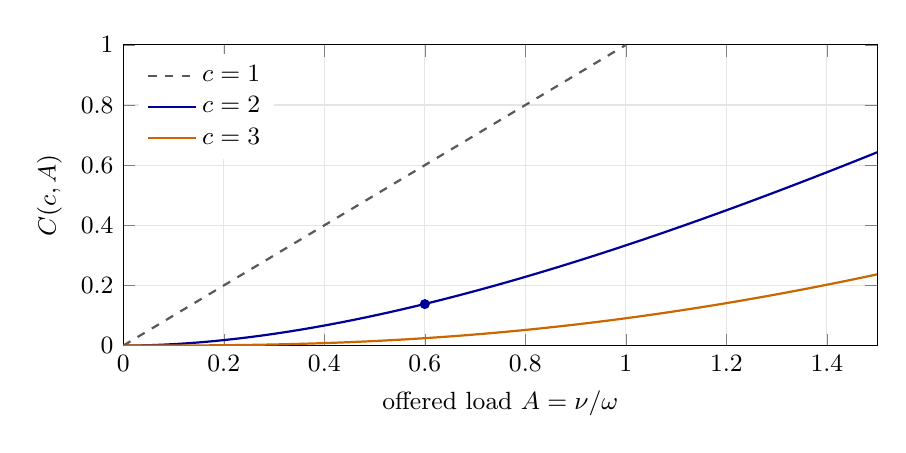
\begin{tikzpicture}
\begin{axis}[
  width=0.92\linewidth, height=5.4cm,
  xlabel={offered load $A = \nu/\omega$}, ylabel={$C(c, A)$},
  xmin=0, xmax=1.5, ymin=0, ymax=1,
  legend style={at={(0.02,0.97)}, anchor=north west, draw=none, fill=white, font=\small},
  grid=major, grid style={gray!20}, tick label style={font=\small}, label style={font=\small}]
  \addplot[gray!70!black, thick, dashed, domain=0:0.999, samples=60] {x};
  \addlegendentry{$c = 1$}
  \addplot[blue!60!black, thick, domain=0:1.5, samples=60] {x^2/(2+x)};
  \addlegendentry{$c = 2$}
  \addplot[orange!80!black, thick, domain=0:1.5, samples=60]
    {(x^3/6*3/(3-x))/(1+x+x^2/2+x^3/6*3/(3-x))};
  \addlegendentry{$c = 3$}
  \addplot[only marks, mark=*, mark size=1.6pt, blue!60!black] coordinates {(0.6,0.138)};
\end{axis}
\end{tikzpicture}
\caption{Probability that a new task waits for a slot, from the Erlang~C
formula \cref{eq:erlang}. The dot marks the example of \cref{sec:agents}.}
\label{fig:erlang}
\end{figure}

\subsection{Selection error}

For the text layer, \cref{fig:drift} already compares the two layouts. In
numbers: with $v = (0.4\,\mathrm{pt})^2$ per glyph, a line of $80$ glyphs has a
mid-line standard deviation of $0.4\sqrt{80/4} \approx 1.8$\,pt from
\cref{eq:bridge} alone, plus the bias of \cref{eq:bias}, which reaches several
points; per-word runs of seven glyphs bound it by $0.4\sqrt{7/4} \approx
0.53$\,pt, well under the width of one letter.
